\documentclass[10pt, table, dvipsnames,xcdraw,handout]{beamer}
\usetheme[progressbar=frametitle]{metropolis}
\usepackage{appendixnumberbeamer}
\usetikzlibrary{arrows.meta, positioning, quotes}
\usepackage[shortlabels]{enumitem}
\usepackage{xcolor}
\usepackage{mathtools}
\usepackage{dsfont}

\usepackage{caption}


\usepackage{cancel}

\newcommand\hcancel[2][black]{\setbox0=\hbox{$#2$}%
\rlap{\raisebox{.45\ht0}{\textcolor{#1}{\rule{\wd0}{1pt}}}}#2} 


\usepackage{booktabs}
\usepackage[scale=2]{ccicons}

\usepackage{pgfplots}
\usepgfplotslibrary{dateplot}

\usepackage{xspace}
\newcommand{\themename}{\textbf{\textsc{metropolis}}\xspace}
\newcommand{\cb}{\cellcolor{blue!25}}


% Notation:
\newcommand{\cT}{\ensuremath{\mathcal{T}}}
\newcommand{\cD}{\ensuremath{\mathcal{D}}}
\newcommand{\cX}{\ensuremath{\mathcal{X}}}
\newcommand{\cY}{\ensuremath{\mathcal{Y}}}
\newcommand{\cZ}{\ensuremath{\mathcal{Z}}}
\newcommand{\cH}{\ensuremath{\mathcal{H}}}
\newcommand{\cG}{\ensuremath{\mathcal{G}}}

\newcommand{\bR}{\ensuremath{\mathbb{R}}}
\newcommand{\bN}{\ensuremath{\mathbb{N}}}
\newcommand{\bP}{\ensuremath{\mathbb{P}}}
\newcommand{\bT}{\ensuremath{\mathbb{T}}}
\newcommand{\bL}{\ensuremath{\mathbb{L}}}

\newcommand{\bfX}{\ensuremath{\mathbf{X}}}
\newcommand{\bfY}{\ensuremath{\mathbf{Y}}}
\newcommand{\bfy}{\ensuremath{\mathbf{y}}}
\newcommand{\bfD}{\ensuremath{\mathbf{D}}}

\def\layersep{2.5cm}

% Tikz seys
\tikzset{cross/.style={cross out, draw, 
         minimum size=2*(#1-\pgflinewidth), 
         inner sep=0pt, outer sep=0pt}}

\title{Machine Learning I}
\subtitle{Lecture 7: Smoothing Methods}
% \date{\today}
\date{}
\author{Nathaniel Bade}
\institute{Northeastern University Department of Mathematics}
% \titlegraphic{\hfill\includegraphics[height=1.5cm]{logo.pdf}}

\begin{document}

\maketitle

\begin{frame}{Table of contents}
  \setbeamertemplate{section in toc}[sections numbered]
  \tableofcontents[hideallsubsections]
\end{frame}


%%%%%%%%%%%%%% Slidshow Start %%%%%%%%%%%%%% 


%Notes: 4 kinds of clusering: Centroid based/kmeans, connecctivity based, density based, distribution based. 
%
% What metrics can we use to evalaute scattering? (internal) Scatter crieteria, silloett coeffcient, (external) mutial information, 
% 
%
% Association rules and merket basket analysis. 
%
%
%
%

\section{Introduction}

\begin{frame}[fragile]{Introduction to Smoothing}
  \begin{minipage}[t][0.5\textheight][t]{\textwidth}
	\centering \includegraphics[width=0.8\textwidth]{L18Phoneme2.png} 
  \end{minipage}
  \vfill
\begin{minipage}[t][0.5\textheight][t]{\textwidth}
A common challenge in data analysis is trying to extract meaning from noisy data. Whether an end in itself or a step in the data processing pipeline, \textbf{smoothing methods} try to extract low variance information from high variance data. 
\end{minipage}
\end{frame}





\begin{frame}[fragile]{Introduction to Smoothing}
  \begin{minipage}[t][0.5\textheight][t]{\textwidth}
	\centering \includegraphics[width=0.8\textwidth]{L18Phoneme2.png} 
  \end{minipage}
  \vfill
\begin{minipage}[t][0.5\textheight][t]{\textwidth}
Consider the Phoneme data above. Whether we are trying to denoise the Frequency/Log-peridogram curve, or fit the frequency to the Log-peridogram, it is not clear that the curve is best represented by a polynomial which must go to $\pm \infty$ at both ends. 
\end{minipage}
\end{frame}


\begin{frame}[fragile]{Introduction to Smoothing}
  \begin{minipage}[t][0.5\textheight][t]{\textwidth}
	\centering \includegraphics[width=0.8\textwidth]{L18Phoneme2.png} 
  \end{minipage}
  \vfill
\begin{minipage}[t][0.5\textheight][t]{\textwidth}
In addition, when we fit polynomials we must fit the parameters globally, while the features we actually care about are local. The degree of a polynomial only specifies the number of local maximuma and minima. Unless the data is specifically expected to have a fixed number of such features, it may be best to fit the features locally, rather than attempt a single global fit. 
\end{minipage}
\end{frame}




\begin{frame}[fragile]{Introduction to Smoothing}
  \begin{minipage}[t][0.5\textheight][t]{\textwidth}
	\centering \includegraphics[width=0.8\textwidth]{L18Phoneme2.png} 
  \end{minipage}
  \vfill
\begin{minipage}[t][0.5\textheight][t]{\textwidth}
Finally, we saw in the last lecture that approximating functions by polynomials, while allowing tighter fitting, may we computationally expensive for large numbers of features. Since RSS itself is the sum of local computations, it usually makes sense to fit nonlinear data not to a single polynomial function, but to a \textbf{smoothing basis}. 
\end{minipage}
\end{frame}








\begin{frame}[fragile]{Introduction to Smoothing}
  \begin{minipage}[t][0.5\textheight][t]{\textwidth}
	\centering \includegraphics[width=0.8\textwidth]{L18Phoneme3.png} 
  \end{minipage}
  \vfill
\begin{minipage}[t][0.5\textheight][t]{\textwidth}
Smoothing is used both in fitting and in preprocessing and feature engineering to construct a useful feature out of a noisy one. \pause It can also be used to split deterministic and Baysean information when the train data spans the entire range $\mathcal{X}$.
\end{minipage}
\end{frame}



\begin{frame}[fragile]{Introduction to Smoothing}
  \begin{minipage}[t][0.5\textheight][t]{\textwidth}
	\centering \includegraphics[width=0.8\textwidth]{L18Datagen.png} 
  \end{minipage}
  \vfill
\begin{minipage}[t][0.5\textheight][t]{\textwidth}
Finally, smoothing methods can be used in data generation by fitting a smoothing surface to a large dataset, modeling the noise, and producing new data as a sum of the smoothed features and sampled noise. 
\end{minipage}
\end{frame}




\begin{frame}[fragile]{Smoothing Procedures}
There are four main views on smoothing mechanisms:
\begin{itemize}
\item[] \textbf{Piecewise smoothing} cuts the domain into regions and models each region separately. \pause
\item[] \textbf{Basis smoothing} attempts to write the data as a weighted sum of basis functions. This will be a unifying theme throughout this lecture. \pause
\item[] \textbf{Kernel smoothing} passes a window over over the data, taking a weighted average of data values near a point. Note: this usage of kernel is not the same as in the kernel method from before. \pause
\item[] \textbf{Dimensional reduction/expansion} attempts to smooth data by passing through a compression or dimensional reduction filter and then projects it back upwards.\pause
\end{itemize}


We will assume unless otherwise stated that $X$ is one dimensional. 
\end{frame}





\section{Piecewise Polynomials and Splines}



\begin{frame}[fragile]{Piecewise Linear Fitting}
  \begin{minipage}[t][0.5\textheight][t]{\textwidth}
	\centering \includegraphics[width=0.8\textwidth]{L18PWL.png} 
  \end{minipage}
  \vfill
\begin{minipage}[t][0.5\textheight][t]{\textwidth}
A piecewise polynomial function $f(X)$ is built by dividing the domain into $K$ disjoint regions $R_k = [\xi_{k-1},\xi_k]$ and representing $f$ by a separate polynomial on each region.  

The set of polynomials on each region will form a \textbf{basis} for the smoothing. 
\end{minipage}
\end{frame}


\begin{frame}[fragile]{Piecewise Linear Fitting}
  \begin{minipage}[t][0.5\textheight][t]{\textwidth}
	\centering \includegraphics[width=0.8\textwidth]{L18PWL.png} 
  \end{minipage}
  \vfill
\begin{minipage}[t][0.5\textheight][t]{\textwidth}
First, lets consider piecewise constant functions $h_k = \mathds{1}_{R_k}$. \pause The least squares estimate of the model
$$
f(X) = \sum_{k=1}^K \beta_k h_k(X)
$$
can be solved by setting $\beta_k = \bar{Y}_k$, the sample mean for each region $R_k$.\pause
\end{minipage}
\end{frame}






\begin{frame}[fragile]{Piecewise Linear Fitting}
  \begin{minipage}[t][0.5\textheight][t]{\textwidth}
	\centering \includegraphics[width=0.8\textwidth]{L18PWL.png} 
  \end{minipage}
  \vfill
\begin{minipage}[t][0.5\textheight][t]{\textwidth}
For a piecewise linear fitting, we need $K$ additional functions in our basis $g_k = X\cdot \mathds{1}_{R_k}$. \pause Fitting
$$
f(X) = \sum_{k=1}^K \beta_k h_k(X) + \gamma_k g_k(X)
$$ 
amounts to performing $K$ linear fits over each region $R_k$. 
\end{minipage}
\end{frame}



\begin{frame}[fragile]{Piecewise Linear Fitting}
  \begin{minipage}[t][0.5\textheight][t]{\textwidth}
	\centering \includegraphics[width=0.8\textwidth]{L18PWL2.png} 
  \end{minipage}
  \vfill
\begin{minipage}[t][0.5\textheight][t]{\textwidth}
Except in special cases we want to impose some boundary conditions on the regions $R_k$. For linear functions the most obvious boundary condition is simple continuity. \pause This leads to $K-1$ conditions
$$
\beta_k + \gamma_k\xi_k = \beta_{k+1} + \gamma_{k+1}\xi_{k+1}\,.
$$\pause
We then have $2K$ parameters and $K-1$ conditions, leaving only $K+1$ basis functions. 
\end{minipage}
\end{frame}


\begin{frame}[fragile]{Piecewise Linear Basis}
  \begin{minipage}[t][0.5\textheight][t]{\textwidth}
	\centering \includegraphics[width=0.8\textwidth]{L18PWL2.png} 
  \end{minipage}
  \vfill
\begin{minipage}[t][0.5\textheight][t]{\textwidth}
Lets define a basis that better incorporates these conditions. Let $h_0(X) = 1$, $h_1(X) = X$ and 
$$
h_{k+1}(X) = (X - \xi_k)_+\,,
$$\pause
where $(X - \xi_k)_+$ denotes the ReLUs function as displayed on the right. \pause We can fit sequentially, first fitting $\beta_0$ and $\beta_1$ to the whole dataset, then $h_\ell$ using feature construction. 
\end{minipage}
\end{frame}




\begin{frame}[fragile]{Fitting Piecewise Linear Basis}
  \begin{minipage}[t][0.5\textheight][t]{\textwidth}
	\centering \includegraphics[width=0.8\textwidth]{L18PWL2.png} 
  \end{minipage}
  \vfill
\begin{minipage}[t][0.5\textheight][t]{\textwidth}
To fit a the piecewise linear basis: 
\begin{itemize}
\item Fit the linear function $\beta_0 + \beta_1 X$ to the whole dataset. \pause
\item Construct the features $X_{k+1} =  (X - \xi_k)_+ - \hat{\beta}_0 + \hat{\beta}_1 X$.\pause
\item Fit the model $\sum_{k=2}^K \beta_k X_{k}$ using linear methods. 
\end{itemize}
\end{minipage}
\end{frame}








\begin{frame}[fragile]{Cubic Splines}
  \begin{minipage}[t][0.5\textheight][t]{\textwidth}
	\centering \includegraphics[width=0.8\textwidth]{L18Cubic2.png} 
  \end{minipage}
  \vfill
\begin{minipage}[t][0.5\textheight][t]{\textwidth}
Moving beyond linear functions, we can enforce continuity on the higher order derivatives. One the left we see a cubic fit with continuous first derivatives and on the right we also impose continuous second derivatives. \pause\newline

A piecewise cubic with continuous second derivatives at the endpoints $\xi$ is called a \textbf{cubic spline}.
\end{minipage}
\end{frame}


\begin{frame}[fragile]{Cubic Splines}
  \begin{minipage}[t][0.5\textheight][t]{\textwidth}
	\centering \includegraphics[width=0.8\textwidth]{L18Cubic2.png} 
  \end{minipage}
  \vfill
\begin{minipage}[t][0.5\textheight][t]{\textwidth}
Using a basis of locally cubic function and enforcing the continuity of the second derivative at the points $\xi_k$ lead to the following basis: $h_0(X) = 1$, $h_1(X)= X$ $h_2(X) = X^2$, $h_3(X) = X^3$, and 
$$
h_{k+3} = (X - \xi_k)_+^3\,.
$$\pause
Note that there are 4K parameters, but we have imposed 3(K-1) conditions.
\end{minipage}
\end{frame}


\begin{frame}[fragile]{Higher Order Splines}
  \begin{minipage}[t][0.5\textheight][t]{\textwidth}
	\centering \includegraphics[width=0.8\textwidth]{L18Cubic2.png} 
  \end{minipage}
  \vfill
\begin{minipage}[t][0.5\textheight][t]{\textwidth}
More generally, an order $M$ spline is a piecewise continuous polynomial with continuous derivatives up to order $M-2$. \pause It can be written in a basis of $K + M$ functions 
$$
h_{k} = X^k\,,k=0,\ldots, M-1\,\hspace{2em} h_{M+\ell -1} = (X-\xi_\ell)^{M-1}\,, \ell=1,\ldots, K\,.
$$\pause
A cubic spline is a order $M=4$ spline. 
\end{minipage}
\end{frame}



\begin{frame}[fragile]{Other Bases}
The cubic spline basis we've described should only be trusted over the regions $R_k$, since outside these regions the boundary cubics quickly go to infinity. \pause 

If data needs to be evaluate outside this fitting region, one may additionally impose linearity at the boundaries. This new basis has four fewer degrees of freedom and can be expressed by the basis $h_0 = 1$, $h_1(X) = X$, 
$$
N_{k+1}(X) = d_k(X) - d_{K-1}(X) 
$$\pause
where
$$
d_k(X) = \frac{(X-\xi_k)_+^3 - (X-\xi_K)_+^3}{\xi_K - \xi_k}\,.
$$\pause

This is called the basis of \textbf{natural cubic splines}.
\end{frame}




\begin{frame}[fragile]{Other Bases}
  \begin{minipage}[t][0.5\textheight][t]{\textwidth}
	\centering \includegraphics[width=0.8\textwidth]{L18Cubic2.png} 
  \end{minipage}
  \vfill
\begin{minipage}[t][0.5\textheight][t]{\textwidth}
Cubic splines are a decent smoothing basis and there is seldom a good reason to go to higher order. However, for a large number of regions it can become computationally inefficient. In this case, there are other spline bases such as \textbf{B-splines} which use the Harr basis to define more computationally efficient spline fittings.
\end{minipage}
\end{frame}


\section{A note on categorical fitting}



\begin{frame}[fragile]{Example: Non-Mixed Features}
  \begin{minipage}[t][0.5\textheight][t]{\textwidth}
	\centering \includegraphics[height=0.5\textheight]{L18ObData.png} 
  \end{minipage}
  \vfill
\begin{minipage}[t][0.5\textheight][t]{\textwidth}
For categorical fitting, we can use smoothing methods to fit the probability discriminant for each category. For example, we can fit the logit probability
$$
\text{logit}[\text{Pr}(G=g|X)] = \theta_0 + h_1(X_1)^T\theta_1+\ldots+h_p(X_p)^T\theta_p\,,
$$\pause
where $h_j$ is a vector of spline basis functions for each feature and $\theta_j$ are a vector of $\beta$'s for each set of splines.  
\end{minipage}
\end{frame}




\begin{frame}[fragile]{Example: Non-Mixed Features}
Combining all of the $h_j$ into one vector $h(X)$ we can write
$$
\text{logit}[\text{Pr}(G=g|X)] = \theta_0 + h_1(X_1)^T\theta_1+\ldots+h_p(X_p)^T\theta_p = h(X)^T\theta\,.
$$\pause
The model has $df_{j} = \sum_{j=1}^p \text{df}_j$ degrees of freedom, where $\text{df}_j$ is the number of basis elements for each variable. Evaluating each basis function at each $X_i$ results in a $N\times \text{df}$ matrix $\mathbf{H}$.\pause

At this point, the problem is like any other and we can proceed to fit it using Newtons method as we did for the linear logistic model. 
\end{frame}


\begin{frame}[fragile]{Example: Non-Mixed Features}
  \begin{minipage}[t][0.5\textheight][t]{\textwidth}
	\centering \includegraphics[height=0.5\textheight]{L18ObData.png} 
  \end{minipage}
  \vfill
\begin{minipage}[t][0.5\textheight][t]{\textwidth}
We can also use standard linear methods like backward subset selection, dropping basis elements according to some metric. In the above, features have been dropped to jointly minimize the training error and the number of degrees of freedom.
\end{minipage}
\end{frame}




\section{Endpoint Selection and Smoothing Splines}

\begin{frame}[fragile]{Smoothing Splines}
In the previous section, our fitting required selecting the endpoints by some procedure that was not specified. While these can be set by hand, spaced linearly according to density and degrees of freedom, or fit as hyperparamters, we want to discuss a way to avoid the problem altogether. \pause

To do so, we minimize
$$
\text{RSS}(f,\lambda) =\sum_{i=1}^N\{y_i - f(x_i)\}^2 + \lambda\int\{f''(t)\}^2\,dt\,
$$
over the (Sobolev) space of functions with finite total integral $\int\{f''(t)\}^2\,dt$. \pause  The parameter $\lambda$ define the smoothness, with $\lambda\to 0$ being any function in the space and $\lambda = \infty$ forcing $f(X)$ linear. 
\end{frame}


\begin{frame}[fragile]{Smoothing Splines}
It can be shown that 
$$
\text{RSS}(f,\lambda) =\sum_{i=1}^N\{y_i - f(x_i)\}^2 + \lambda\int\{f''(t)\}^2\,dt\,
$$
has a unique, finite dimensional minimizer given by a basis of natural cubic splines
$$
f(X) = \sum_{j=1}^N N_j(X)\theta_j\,,
$$\pause
with regions defined to have endpoint at the datapoints $x_i$. \pause The penalty $\lambda$ becomes a dampening of the coefficients, which reduces the potential overfitting.
\end{frame}



\begin{frame}[fragile]{Smoothing Splines}
Writing
$$
\Omega_{jk} = \int N''_j(t)N''_k(t)\,dt\,\hspace{2em} \{\mathbf{N}\}_{ij} = N_j(X_i)\,,
$$\pause
the loss
$$
\text{RSS}(f,\lambda) =\sum_{i=1}^N\{y_i - f(x_i)\}^2 + \lambda\int\{f''(t)\}^2\,dt\,
$$
can be written as
$$
\text{RSS}(f,\lambda) = (\bfy - \mathbf{N}\theta)^T(\bfy - \mathbf{N}\theta) + \lambda\theta^T\Omega\theta\,.
$$\pause
It can then be solved for
$$
\hat{\theta} = (\mathbf{N}^T\mathbf{N} + \lambda\Omega)^{-1}\mathbf{N}^T\bfy\,.
$$
To be clear, the basis $N_i(x)$ is known explicitly, so this is just a generalized ridge regression problem.
\end{frame}



\begin{frame}[fragile]{Example: Non-Mixed Features}
  \begin{minipage}[t][0.5\textheight][t]{\textwidth}
	\centering \includegraphics[height=0.5\textheight]{L18CubicSpline.png} 
  \end{minipage}
  \vfill
\begin{minipage}[t][0.5\textheight][t]{\textwidth}
For example, we see the smoothing spline fit to the data from before for different values of $\lambda$. In this case, relatively close lambda values actually give a significantly different interpolation. 
\end{minipage}
\end{frame}




\begin{frame}[fragile]{Degrees of Freedom for Smoothing Splines}
As a function of $\lambda$, a smoothing spline is a \textbf{linear smoother} since the parameters are linear functions of $y_i$. \pause Indeed, after fitting
$$
\hat{f} = \mathbf{N}(\mathbf{N}^T\mathbf{N} + \lambda\Omega)^{-1}\mathbf{N}^T\bfy = \mathbf{S}_\lambda \bfy\,,
$$
where $\mathbf{S}_\lambda$ is a linear operator known as the \textbf{smoother matrix}.\pause

If we fit cubic splines with $M<N$ endpoints $\xi$ as in last section, we can form a similar $N\times M$ projection matrix $\mathbf{B}_\xi$ and solve the least squares problem by
$$
\hat{f} = \mathbf{B}_\xi(\mathbf{B}_\xi^T\mathbf{B}_\xi)^{-1}\mathbf{B}_\xi^T \mathbf{y} = \mathbf{H}_\xi \bfy\,.
$$
\end{frame}



\begin{frame}[fragile]{Degrees of Freedom for Smoothing Splines}
Both $\mathbf{S}_\lambda$ and $\mathbf{H}_\xi$ are symmetric and positive definite. In addition, $\mathbf{H}_\xi^2 = \mathbf{H}_\xi$ is idempotent, while $\mathbf{S}_\lambda^2 \preceq \mathbf{S}_\lambda$, that is $\mathbf{S}_\lambda^2$ exceed itself by a positive semidefinite matrix. \pause

The trace of an idempotent is its rank so for generic $\xi$, $M = \text{tr}(\mathbf{H}_\xi)$ gives then number of basis functions or degrees of freedom. By analogy, we define the effective degrees of freedom of  $\mathbf{S}_\lambda$ to be $\text{df}_\lambda = \text{tr}(\mathbf{S}_\lambda)$.\pause 

We will say a few words to justify this, and describe the smoothing behavior.
\end{frame}



\begin{frame}[fragile]{Degrees of Freedom for Smoothing Splines}
Notice that, for $\mathbf{K} =  (\mathbf{N}^T)^{-1}\Omega\mathbf{N}$, 
$$
\mathbf{S}_\lambda = \mathbf{N}(\mathbf{N}^T\mathbf{N} + \lambda\Omega)^{-1}\mathbf{N}^T = (1+\lambda\mathbf{K})^{-1}\,
$$\pause 
so $\hat{f} = \mathbf{S}_\lambda\bfy$ minimizes
$$
(\bfy - {f})^T(\bfy - {f}) + \lambda f^T\mathbf{K}f\,.
$$\pause 
If the penalty matrix $\mathbf{K}$ has eigenvalues $d_k$, we can decompose $\mathbf{S}_\lambda \bfy$ as
$$
\mathbf{S}_\lambda\bfy = \sum_{i=1}^N\frac{1}{1+\lambda d_k}\mathbf{u}_i\langle\mathbf{u}_i,\bfy\rangle\,.
$$\pause
Note, $\mathbf{S}_\lambda$ has the same Eigenvectors regardless of $\lambda$, all $\lambda$ is doing is dampening them proportional to the eigenvalues $d_i$. \pause In addition, as $\lambda\to \infty$, $\text{df}$ decreases from $N$ to 2, since $\mathbf{K}$ can be shown to have 2 zero eigenvalues. 
\end{frame}



\begin{frame}[fragile]{Degrees of Freedom for Smoothing Splines}
  \begin{minipage}[t][0.5\textheight][t]{\textwidth}
	\centering \includegraphics[height=0.5\textheight]{L18SmoothingMatrix.png} 
  \end{minipage}
  \vfill
\begin{minipage}[t][0.5\textheight][t]{\textwidth}
Here we see a smoothing matrix $\mathbf{S}_\lambda$ ordered so that $x_i<x_{i+1}$. The expressions on the matrix correspond to points projected onto the basis and imply that smoothing splines are a local method.
\end{minipage}
\end{frame}


\section{Multidimensional Splines}

\begin{frame}[fragile]{Multidimensional Splines}
The multivariate case follows directly from the one variable case. \pause For example, in $\mathbb{R}^2$, if $h_{1i}$ is a spline basis for $X_1$, and $h_{2j}$ form a spline basis for $X_2$, we can form the tensor product basis
$$
g_{ij}(X)  = g_{ij}(X_1,X_2) = h_{1i}(X_1)h_{2j}(X_2)\,.
$$\pause
We can then fit 
$$
g(X) = \sum_{i=1}^{M_1}\sum_{j=1}^{M_2} g_{ij}(X)^T\theta_{ij} = g(X)^T\theta\,,
$$
for a suitably reshaped $g(X)$ and $\theta$.
\end{frame}


\begin{frame}[fragile]{Multidimensional Splines}
  \begin{minipage}[t][0.5\textheight][t]{\textwidth}
	\centering \includegraphics[height=0.5\textheight]{L18BloodPressure.png} 
  \end{minipage}
  \vfill
\begin{minipage}[t][0.5\textheight][t]{\textwidth}
In practice, the only difficulty is picking the lattice. For a maximum number of degrees of freedom $M$, one can separate the domain into a lattice of $M$ points and then throw away all points outside the convex hull of the dataset. 
\end{minipage}
\end{frame}



\begin{frame}[fragile]{Multidimensional Smoothing Splines}
For smoothing splines, we now need to minimize a function of the form
$$
RSS(\theta) = \sum_{i=1}^N(y_i - f(x_i))^2 + \lambda\int_{\mathbb{R}^2} \left( \frac{\partial}{\partial x_1} + \frac{\partial}{\partial x_2}\right)^2 f(x)\,dx_1\,dx_2\,.
$$\pause 
The solutions are smooth 2d surfaces known as \textbf{thin plate splines}, and take the form of radial basis functions
$$
h_i(X) = ||X-X_i||^2\log||X - X_i||\,.
$$
As before, for $\lambda = 0$ the solution approaches an interpolating function and for $\lambda\to \infty$, the solution approaches the least squares plane. 
\end{frame}




\section{Kernel Smoothing}

\begin{frame}[fragile]{Nearest Neighbor Kernel Smoothing}
  \begin{minipage}[t][0.5\textheight][t]{\textwidth}
	\centering \includegraphics[height=0.5\textheight]{L18KernelSmoothing.png} 
  \end{minipage}
  \vfill
\begin{minipage}[t][0.5\textheight][t]{\textwidth}
Another way to smooth functions locally is to apply a filter to each point. The simplest kernel smoothing filter is to simply compute the average value of $k$ nearest training points $N_k(x)$ :
$$
\hat{f}(X) = \text{Avg}(y_i|x_i\in N_k(x))
$$\pause
However, this results in the bumpy discontinuous curve on the left. 
\end{minipage}
\end{frame}


\begin{frame}[fragile]{Nearest Neighbor Kernel Smoothing}
  \begin{minipage}[t][0.5\textheight][t]{\textwidth}
	\centering \includegraphics[height=0.5\textheight]{L18KernelSmoothing.png} 
  \end{minipage}
  \vfill
\begin{minipage}[t][0.5\textheight][t]{\textwidth}
A more sophisticated smoothing involves weighting the points so that further points contribute less. For example, we take the average
$$
\hat{f}(x) = \frac{\sum_{i=1}^N K_\lambda(x,x_i)y_i}{\sum_{i=1}^N K_\lambda(x,x_i)}\,,\hspace{1em} K_\lambda(x,x_i) = D\left(\frac{|x-x_0|}{\lambda}\right)\,
$$\pause
where $D(t) = \frac34(1-t^2)$ for $|t|\leq1$ is the Epanechnikov kernel. 
\end{minipage}
\end{frame}


\begin{frame}[fragile]{Nearest Neighbor Kernel Smoothing}
  \begin{minipage}[t][0.5\textheight][t]{\textwidth}
	\centering \includegraphics[height=0.5\textheight]{L18KernelSmoothing.png} 
  \end{minipage}
  \vfill
\begin{minipage}[t][0.5\textheight][t]{\textwidth}
The Epanechnikov kernel fits a continuous function to the data. The \textbf{bandwidth} $\lambda$ determines the window size and can be constant, depend on $k$-neighborhood size $\lambda = h_\lambda(X) = |X - X_{[k]}|$, or vary according to other considerations.
\end{minipage}
\end{frame}



\begin{frame}[fragile]{Nearest Neighbor Kernel Smoothing}
  \begin{minipage}[t][0.5\textheight][t]{\textwidth}
	\centering \includegraphics[height=0.5\textheight]{L18KernelSmoothing.png} 
  \end{minipage}
  \vfill
\begin{minipage}[t][0.5\textheight][t]{\textwidth}
In general, a kernel has finite support $K(x,x_i) = 0$ for $|x-x_i|\geq1$, symmetry $K(-x,-x_i) = K(x,x_i)$ and positivity $K(x,x_i)>0$ for $|x-x_i|<1$. All of the following results will hold for such kernels. 
\end{minipage}
\end{frame}



\begin{frame}[fragile]{Practical concerns}
There are a couple of consideration in practice:
\begin{itemize}
\item[] For fixed $\lambda$, large $\lambda$ implies low variance since we're averaging over more data points but higher bias. \pause
\item[] For density based $\lambda$, the bias tends to be constant but the variance is inverse proportional to the local density.\pause
\item[] The neighborhood of the boundary tends to contain fewer points, and so our estimates will be less accurate there. \pause
\item[] We have to select a kernel. The Epanechnikov kernel can be replaced by a Gaussian kernel for example, giving slightly different fitting. 
\end{itemize}

\end{frame}



\begin{frame}[fragile]{Locally Linear Regression}
  \begin{minipage}[t][0.5\textheight][t]{\textwidth}
	\centering \includegraphics[height=0.5\textheight]{L18NWEst.png} 
  \end{minipage}
  \vfill
\begin{minipage}[t][0.5\textheight][t]{\textwidth}
The boundary value problem, and indeed some internal variance, can be solved by replacing the pointwise estimate with a linear estimate called \textbf{local linear regression}. 
\end{minipage}
\end{frame}


\begin{frame}[fragile]{Locally Weighted Regression}
Local linear regression attempts to solve a separate weighted least squared problem at each target point $x_0$. The local loss is a function
$$
RSS = \sum_{i=1}^N K_\lambda(x_0,x_i)[y_i - \alpha_{x_0} - \beta_{x_0}x_i]^2\,,
$$\pause
where $\alpha_{x_0}$ and  $\beta_{x_0}$ are constants. \pause The fit is then $\hat{f}(x_0) = \hat{\alpha}_{x_0} + \hat{\beta}_{x_0}x_0$, and is uniquely determined for the point $x_0$. \pause

Letting $\mathbf{X} = (1,x_i)$ be the matrix with a column of 1's and a column of data points $x_i$ as usual and let $\mathbf{W}(x_0)$ be diagonal with entries $K_\lambda(x_0,x_i)$. Then
$$
\hat f(x_0) = [1,x_0]^T(\mathbf{X}^T\mathbf{W}(x_0)\mathbf{X})^{-1}\bfX^T\mathbf{W}(x_0) \bfy = \sum_{i=1}^N\ell_i(x_0)y_i\,.
$$
\end{frame}



\begin{frame}[fragile]{Locally Linear Regression}
  \begin{minipage}[t][0.5\textheight][t]{\textwidth}
	\centering \includegraphics[height=0.5\textheight]{L18LLR.png} 
  \end{minipage}
  \vfill
\begin{minipage}[t][0.5\textheight][t]{\textwidth}
In the figure above, we see the weights $\ell_i(x_0)$ for different $x_0$ as we move through the dataset. 
\end{minipage}
\end{frame}



\begin{frame}[fragile]{Kernel Carpentry}
Assume for a moment that the labels are generated by $y_i = f(x_i)  + \epsilon$, where $f$ is twice differentiable. It turns out the local linear regression exactly matches the function $f(x)$ up to first order. \pause With a bit of work one can show that
$$
\sum_{i}\ell_i(x_0) = 1\,,\hspace{2em} \sum_i^N(x_i - x_0)\ell_i(x_0) = 0
$$
provided $K$ is a kernel in the sense defined before. \pause Expanding $f$ around $x_0$,
$$
E[\,\hat{f}(x_0) \,]= f(x_0)\sum_{i=1}^N\ell_i(x_0) + f'(x_0)\sum_{i=1}^N\ell_i(x_0) (x_i-x_0) + \text{h.o.t.}\,.
$$\pause
But the conditions above mean that 
$$
\hat{f}(x_0) = f(x_0) + \frac12f''(x_0)\sum_{i=1}^N\ell_i(x_0) (x_i-x_0) ^2 + R\,,
$$
so up to linear order the the local regression exactly matches the true function. 
\end{frame}




\begin{frame}[fragile]{Kernel Carpentry}
The result
$$
\hat{f}(x_0) = f(x_0) + \frac12f''(x_0)\sum_{i=1}^N\ell_i(x_0) (x_i-x_0) ^2\,,
$$
can be rewritten 
$$
\text{Bias}[\hat{f}(x_0)] = \hat{f}(x_0) - f(x_0)  = \frac12f''(x_0)\sum_{i=1}^N\ell_i(x_0) (x_i-x_0) ^2 + R\,,
$$
and we say the local bias is of quadratic order. \pause This is the same as saying that locally we have fit the function exactly up to linear order. This result is known as \textbf{automatic kernel carpentry}.
\end{frame}





\begin{frame}[fragile]{Local Polynomial Regression}
  \begin{minipage}[t][0.5\textheight][t]{\textwidth}
	\centering \includegraphics[height=0.5\textheight]{L18LQR.png} 
  \end{minipage}
  \vfill
\begin{minipage}[t][0.5\textheight][t]{\textwidth}
Higher degree polynomials account for higher degrees of bias, but they of course come with a tradeoff in variance. The local polynomial problem is to minimize
$$
RSS = \sum_{i=1}^NK(x_0,x_i) \left( y_i - \alpha_{x_0} - \sum_{j=1}^d \beta_{x_0,j}x_i^j \right)\,.
$$
\end{minipage}
\end{frame}



\begin{frame}[fragile]{Local Polynomial Regression}
  \begin{minipage}[t][0.5\textheight][t]{\textwidth}
	\centering \includegraphics[height=0.5\textheight]{L18LQR.png} 
  \end{minipage}
  \vfill
\begin{minipage}[t][0.5\textheight][t]{\textwidth}
In the figure above, we see that local linear fits exhibit their bias in regions of high curvature, while degree 2 polynomials can correct this. \pause In general it is very nongeneric to have a point that is dominated by behavior of order higher than 2, so we can usually stop at local quadratic regression. 
\end{minipage}
\end{frame}




\begin{frame}[fragile]{Selecting the Kernel Width}
The bias-variance tradeoff is controlled by the bandwidth $\lambda$, where $\lambda$ acts as the cutoff for the Epanechnikov kernel, the standard deviation for the Gaussian kernel, or number of neighbors for the $k$ nearest neighbors kernel. \pause

Local regression smoothers are linear estimates, and so can be expressed by the smoother matrix $\hat f =\mathbf{S}_\lambda\bfy$, where $\{\mathbf{S}_\lambda\}_{ij} = \ell_i(x_j)$. \pause The effective number of degrees of freedom can then be calculated by
$$
\text{df}_\lambda = \text{tr}(\mathbf{S}_\lambda)\,.
$$
\end{frame}




\begin{frame}[fragile]{Kernels in Higher Dimensions}
For higher dimensional kernel fitting, we again want to fit a dataset to a set of degree $d$ polynomials. For example, for two features $(X_1,X_2)$, let $b(X) = (1,X_1,X_2,X_1^2,X_1X_2,X_2^2)$\, and consider minimizing
$$
RSS = \sum_{i=1}^NK_\lambda(x_0,x_i)(y_i - b^T(x_i)\beta_{x_0})
$$\pause
In the kernel, we typically replace evenness with radial symmetry, such as in the radial Epanechnikov function
$$
K_\lambda(x_0,x) = D\left(\frac{||x-x_0||}{\lambda}\right)\,.
$$\pause 
The main issue for high dimensional smoothing is curse of dimensionally, which here means that an increasing percentage of the points will be boundary points. \pause Even local linear regression becomes useless in dimensions much above 3, but higher order polynomial techniques can still be effective. 
\end{frame}



\section{Other Bases}


\begin{frame}[fragile]{Other Bases}
There are a few other bases we should mention.

\begin{itemize}
\item[] \textbf{Fourier Basis:} The canonical basis for wavelike data, separates waves into sums of frequencies.\pause 
\item[] \textbf{Wavelet Bases:} Any of a family of bases that consist of ``waves'' of a finite length. Unlike the Fourier basis this gives them both frequency and locality. \pause
\item[] \textbf{Haar Basis:} A computationally efficient wavelet basis composed of piecewise step functions that cover a partition of the domain. \pause
\item[] \textbf{BSpline Basis:} Polynomial combinations of the Haar basis functions that provide a differenitable spline basis. The Bspline basis is what is typically used in actual spline computation. 
\end{itemize}
\end{frame}



\begin{frame}[fragile]{Fourier Basis}
  \begin{minipage}[t][0.5\textheight][t]{\textwidth}
	\centering \includegraphics[height=0.5\textheight]{L18Fourier.png} 
  \end{minipage}
  \vfill
\begin{minipage}[t][0.5\textheight][t]{\textwidth}
The Fourier basis transforms repeating waves into sums of sine and cosine functions at different frequencies:
$$
f(x) = \sum_{n=0}^\infty 	a_n\sin(2\pi n/T) + b_n\cos(2\pi n/T) \,.
$$\pause
It is important to note that the Fourier basis truncated to a finite number of terms is inherently non-local. 
\end{minipage}
\end{frame}



\begin{frame}[fragile]{Wavelet Basis}
  \begin{minipage}[t][0.5\textheight][t]{\textwidth}
	\centering \includegraphics[width=0.8\textwidth]{L18Wavelets.png} 
  \end{minipage}
  \vfill
\begin{minipage}[t][0.5\textheight][t]{\textwidth}
A wavelet basis is a basis of functions that try to capture both frequency and location. There are many adapted to various theoretical and practical uses, and are particularly used in image processing and storage. 
\end{minipage}
\end{frame}



\begin{frame}[fragile]{Haar Basis}
  \begin{minipage}[t][0.5\textheight][t]{\textwidth}
	\centering \includegraphics[width=0.8\textwidth]{L18Haar.png} 
  \end{minipage}
  \vfill
\begin{minipage}[t][0.5\textheight][t]{\textwidth}
One of the building blocks of computationally efficient wavelet computations is the Haar basis.  We construct the basis recursively, starting with a constant function $h_0(x)$ on a bounded domain, for example $R = [0,1]$. \pause Then,
$$
h_1(x) = \begin{cases}
1&\text{for } x<\frac12\,,\\
-1&\text{for }x\geq \frac12\,.
\end{cases}
$$\pause
$h_0$ and $h_1$ are orthogonal. We continue cutting each domain in half. 
\end{minipage}
\end{frame}




\begin{frame}[fragile]{B-Spline Basis}
  \begin{minipage}[t][0.5\textheight][t]{\textwidth}
	\centering \includegraphics[width=0.4\textwidth]{L18Bsplines.png}\includegraphics[width=0.4\textwidth]{L18Bsplines2.png} 
  \end{minipage}
  \vfill
\begin{minipage}[t][0.5\textheight][t]{\textwidth}
B-splines are defined recursively from a Haar like basis. Letting $B_{i,k}(x) = \mathds{1}_{R_k}(x)$, the order $m$ spline is 
$$
B_{i,m}(x) = \frac{x - \xi_i}{\xi_{i+m-1}-\xi_i}B_{i,m-1}(x) + \frac {\xi_{i+m} - x}{\xi_{i+m}-\xi_{i+1}}B_{i+1,m-1}(x)
$$
\end{minipage}
\end{frame}



\begin{frame}[fragile]{B-Spline Basis}
  \begin{minipage}[t][0.5\textheight][t]{\textwidth}
	\centering \includegraphics[width=0.4\textwidth]{L18Bsplines.png}\includegraphics[width=0.4\textwidth]{L18Bsplines2.png} 
  \end{minipage}
  \vfill
\begin{minipage}[t][0.5\textheight][t]{\textwidth}
The recursive nature of the construction allows for much faster smoothing by B-splines of order 4 than by normal cubic splines. For a large number $N$ of regions, fitting by cubic splines can be shown to be $O(N^3)$ while under mild sparsity conditions fitting by B-splines is of order $O(N)$.
\end{minipage}
\end{frame}



\begin{frame}[fragile]{Reference}
The main reference for this lecture is ESLII Chapters 5 and 6. 

The following reference summarizes many results for local linear regression: \url{http://courses.ieor.berkeley.edu/ieor265/lecture_notes/ieor265_lec6.pdf}

Wavelet Gallery picture taken from \url{https://www.intechopen.com/books/wavelet-transform-and-some-of-its-real-world-applications/empirical-wavelet-transform-based-detection-of-anomalies-in-ulf-geomagnetic-signals-associated-to-se}
\end{frame}



\end{document}

%%%%%%%%%%%%%%%%%%%%%%%%%%%%%%%%%%
%
% |   __|___ _| |  |    \ ___ ___ _ _ _____ ___ ___| |_ 
% |   __|   | . |  |  |  | . |  _| | |     | -_|   |  _|
% |_____|_|_|___|  |____/|___|___|___|_|_|_|___|_|_|_|                                                   
%
%%%%%%%%%%%%%%%%%%%%%%%%%%%%%%%%%%



%%%%%%%%%%%%%%%%%%%%%%%%%%%%%%%%%%%%%%%%%%%
%%%%%%%%%%%%%%%%%%%%%%%%%%%%%%%%%%%%%%%%%%%
%%%%%%%%%%%%%%%%%%%%%%%%%%%%%%%%%%%%%%%%%%%



\begin{frame}[fragile]{Introduction}

\end{frame}




\begin{frame}[fragile]{Binary Classification}
  \begin{minipage}[t][0.5\textheight][t]{\textwidth}
	\centering \includegraphics[height=0.5\textheight]{.png} 
  \end{minipage}
  \vfill
\begin{minipage}[t][0.5\textheight][t]{\textwidth}

\end{minipage}
\end{frame}



\begin{frame}[fragile]{Test}
\begin{minipage}[t][0.5\textheight][t]{\textwidth}\centering
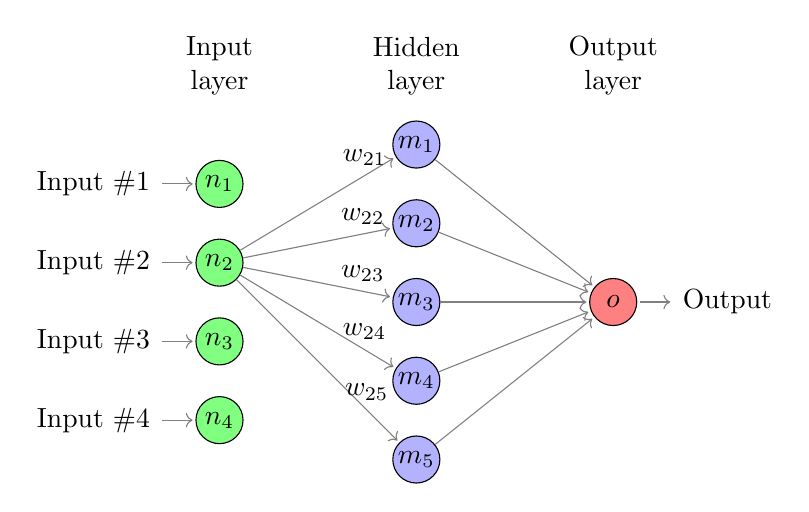
\begin{tikzpicture}[shorten >=1pt,->,draw=black!50, node distance=\layersep]
%https://tex.stackexchange.com/questions/96846/how-to-place-label-in-middle-of-line-above-and-below-with-tikz
    \tikzstyle{every pin edge}=[<-,shorten <=1pt]
    \tikzstyle{neuron}=[circle,fill=black!25,minimum size=17pt,inner sep=0pt, draw=black]
    \tikzstyle{input neuron}=[neuron, fill=green!50];
    \tikzstyle{output neuron}=[neuron, fill=red!50];
    \tikzstyle{hidden neuron}=[neuron, fill=blue!30];
    \tikzstyle{annot} = [text width=4em, text centered]

    % Draw the input layer nodes
    \foreach \name / \y in {1,...,4}
    % This is the same as writing \foreach \name / \y in {1/1,2/2,3/3,4/4}
        \node[input neuron, pin=left:Input \#\y] (I-\name) at (0,-\y) {$n_\y$};

    % Draw the hidden layer nodes
    \foreach \name / \y in {1,...,5}
        \path[yshift=0.5cm]
            node[hidden neuron] (H-\name) at (\layersep,-\y cm) {$m_\y$};

    % Draw the output layer node
    \node[output neuron,pin={[pin edge={->}]right:Output}, right of=H-3] (O) {$o$};

    % Connect every node in the input layer with every node in the
    % hidden layer.
%    \foreach \source in {1,...,4}
%        \foreach \dest in {1,...,5}
%            \draw (I-\source) -- node[below] {$w_ij$} ++ (H-\dest);


%    \foreach \source in {1,...,4}
        \foreach \dest in {1,...,5}
            \draw (I-2) -- node[above, pos=0.8] {$w_{2\dest}$} ++ (H-\dest);

    % Connect every node in the hidden layer with the output layer
    \foreach \source in {1,...,5}
        \path (H-\source) edge (O);

    % Annotate the layers
    \node[annot,above of=H-1, node distance=1cm] (hl) {Hidden layer};
    \node[annot,left of=hl] {Input layer};
    \node[annot,right of=hl] {Output layer};
\end{tikzpicture}
  \end{minipage}
  \vfill
\begin{minipage}[t][0.5\textheight][t]{\textwidth}

\end{minipage}


\end{frame}




\begin{frame}[fragile]{Point Variance of Linear Predictor}

\begin{align*}
\action<+->{ &=&&}
\\
\action<+->{  &=   && }
\end{align*}
\action<+->{The}
\end{frame}



\begin{frame}[fragile]{Correlation}
\begin{itemize}
\item[] \textbf{Serial No.} is basically uncorrelated with anything. \pause
\item[] \textbf{Admit} is highly correlated with \textbf{CGPA}, \textbf{TOEFL Score} and \textbf{GRE Score}\pause
\item[] \textbf{Research} has a lowish correlation with \textbf{Admit}, but also with everything else.  
\end{itemize}
\end{frame}











\begin{frame}[fragile]{Bias, Variance and Parameters}
  \begin{minipage}[t][0.5\textheight][t]{\textwidth}
	\centering
	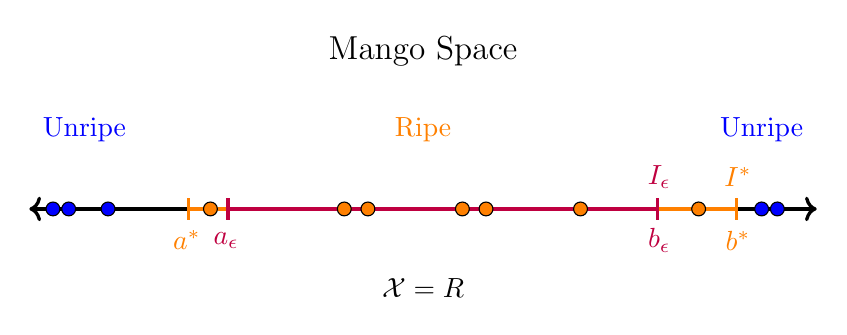
\begin{tikzpicture}
		\draw[<->,very thick] (-5,0) -- (5,0);
		\draw[color = orange, |-|,very thick] (-3,0) -- (4,0);
		\node[color=orange] at (4,.4) {$I^*$};
		\node at (0,2) {\large Mango Space} ;
		\node at (0,-1) {$\mathcal{X} = \mathbb{R}$} ;
		\node [color=blue] at (-4.3,1) {Unripe} ;
		\node [color=blue] at (4.3,1) {Unripe} ;
		\node [color=orange] at (0,1) {Ripe} ;

		\node [color=orange] at (-3,-.4) {$a^*$} ;
		\node [color=orange] at (4,-.4) {$b^*$} ;

		\draw [color=purple, |-|,very thick] (-2.5,0) -- (3,0);
		\node [color=purple] at (3,.4) {$I_\epsilon$} ;
		\node [color=purple] at (-2.5,-.4) {$a_\epsilon$} ;
		\node [color=purple] at (3,-.4) {$b_\epsilon$} ;

%		\draw [color=olive, |-|,very thick] (-3.5,0) -- (2.5,0);
%		\node [color=olive] at (3,.4) {$h_{\mathcal{T}}$} ;



		\node[circle,draw=black, fill=orange, inner sep=0pt,minimum size=5pt] at (2,0) {};
		\node[circle,draw=black, fill=orange, inner sep=0pt,minimum size=5pt] at (-1,0) {};
		\node[circle,draw=black, fill=orange, inner sep=0pt,minimum size=5pt] at (-.7,0) {};
		\node[circle,draw=black, fill=orange, inner sep=0pt,minimum size=5pt] at (.5,0) {};
		\node[circle,draw=black, fill=orange, inner sep=0pt,minimum size=5pt] at (.8,0) {};
		\node[circle,draw=black, fill=orange, inner sep=0pt,minimum size=5pt] at (-2.7,0) {};
		\node[circle,draw=black, fill=orange, inner sep=0pt,minimum size=5pt] at (3.5,0) {};

		\node[circle,draw=black, fill=blue, inner sep=0pt,minimum size=5pt] at (-4.5,0) {};
		\node[circle,draw=black, fill=blue, inner sep=0pt,minimum size=5pt] at (-4,0) {};
		\node[circle,draw=black, fill=blue, inner sep=0pt,minimum size=5pt] at (-4.7,0) {};
		\node[circle,draw=black, fill=blue, inner sep=0pt,minimum size=5pt] at (4.3,0) {};
		\node[circle,draw=black, fill=blue, inner sep=0pt,minimum size=5pt] at (4.5,0) {};
	\end{tikzpicture}
  \end{minipage}
  \vfill
  \begin{minipage}[t][0.5\textheight][t]{\textwidth}
Lets understand this visually.
$$
Err(x_0) = \sigma_\epsilon^2 + [E_\cT[\hat f(x_0)] - f(x_0)]^2 + E_\cT\big[ \hat{f}(x_0) - E_\cT[\hat{f}(x_0)] \big]^2\,.
$$\pause
Consider a data set, 
\end{minipage}
\end{frame}





























